\section{Course concepts used in the implementation}
\label{app:course}

\begin{table}[H]
\centering
\small
\caption{Where course concepts (Lectures 1--8) appear in the code base.}
\begin{tabular}{p{1.4cm}p{6.6cm}p{6.4cm}}
\toprule
Lecture & Concept & Implementation \\
\midrule
L1 & Reproducible seeding; scaler fitted on training data only & \texttt{src/utils.py}; per-lead standardiser in \texttt{src/data.py} \\
L2--L3 & 1-D convolution, stride, padding; layer summaries & ResNet1d and convolutional stems; \texttt{torchinfo} summaries \\
L4 & RNN/LSTM; BCE with logits; class weighting; gradient clipping; early stopping with deep-copied best weights & CNN-BiLSTM and vanilla-RNN ablation; \texttt{run\_epoch}/\texttt{train\_model} in \texttt{src/train.py} \\
L5 & Controlled comparison; majority/prior baseline; receptive field; CNN + recurrent hybrid & E1/E1b design; B0; receptive-field sweep (kernel 3--31); CNN-BiLSTM \\
L6 & Hand-written query/key/value attention; residual + LayerNorm; positional encoding & \texttt{MultiHeadSelfAttention} and pre-LN blocks in \texttt{src/models.py} \\
L7 & Vision Transformer: patches, CLS token, sinusoidal encoding; AdamW; TensorBoard & ECG-ViT; optimiser and logging in \texttt{src/train.py} \\
L8 & ResNet; transfer learning with discriminative learning rates; ensembles; Grad-CAM (including for Transformers) & S2 transfer; seed and heterogeneous ensembles; \texttt{src/gradcam.py} \\
\bottomrule
\end{tabular}
\end{table}

\section{Hyper-parameters}
\label{app:hparams}

\begin{table}[H]
\centering
\small
\caption{Shared training settings (identical for all supervised models).}
\begin{tabular}{ll}
\toprule
Setting & Value \\
\midrule
Input & 100\,Hz, 10\,s (1,000 samples), per-lead z-score from training fold \\
Loss & binary cross-entropy with logits (class weighting only in the E1b ablation) \\
Optimiser & AdamW, learning rate $10^{-3}$, weight decay $10^{-2}$ \\
Schedule & one-cycle, 10\% warm-up \\
Batch size / max epochs & 128 / 50 \\
Early stopping & validation macro AUROC, patience 10, best weights restored \\
Gradient clipping & global norm 1.0 \\
Augmentation & amplitude scale $\sigma=0.1$, offset $\sigma=0.05$, noise $\sigma=0.02$, circular shift $\pm0.5$\,s \\
Transfer (S2) & backbone learning rate $\times0.1$ (fine-tune) or frozen \\
LA-ResNet (S3) & full 12 leads 0.5, reduced configuration 0.3, random subset 0.2 \\
MSM pre-training (S4) & 8/50 patches masked, MSE on masked patches, $\leq$100 epochs, patience 10 \\
Seeds & 0, 1, 2 (ablations and label-efficiency runs: seed 0) \\
Hardware & NVIDIA RTX 3060 Laptop GPU (6\,GB), mixed precision \\
\bottomrule
\end{tabular}
\end{table}

\section{Ablations}
\label{app:ablation}

\begin{table}[H]
\centering
\small
\caption{Single-seed ablations on 12 leads (seed 0, test macro AUROC). Differences of this size are comparable to the across-seed spread and are not interpreted as evidence that one variant is better.}
\begin{tabular}{lc}
\toprule
Variant & Macro AUROC \\
\midrule
ResNet1d (reference, kernel 7) & 0.9211 \\
ResNet1d without residual connections & 0.9166 \\
ResNet1d kernel 3 / 15 / 31 & 0.9233 / 0.9187 / 0.9152 \\
ResNet1d with class-weighted loss & 0.9242 \\
CNN-BiLSTM (LSTM) & 0.9258 \\
CNN-BiLSTM with vanilla RNN & 0.9279 \\
\bottomrule
\end{tabular}
\end{table}

\begin{figure}[H]
\centering
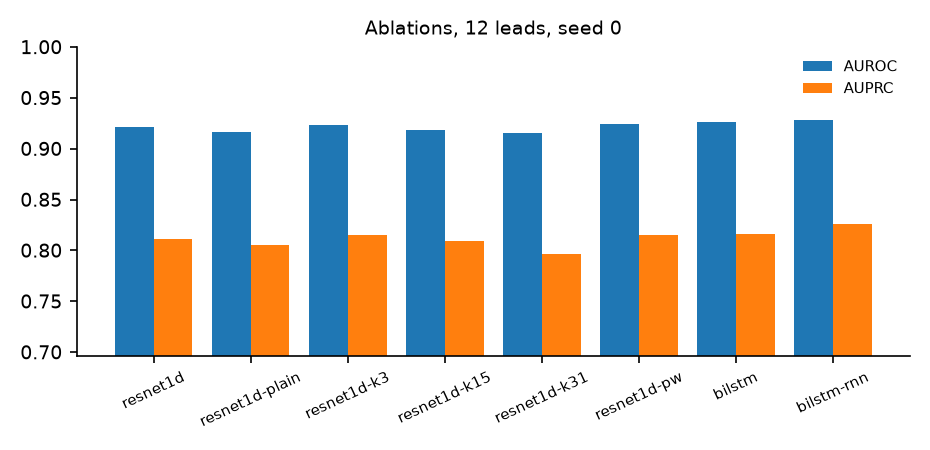
\includegraphics[width=0.7\linewidth]{fig9_ablations.png}
\caption{Ablations on 12 leads (seed 0): macro AUROC and AUPRC.}
\end{figure}

\section{Subgroups}
\label{app:subgroups}

\begin{table}[H]
\centering
\small
\caption{Macro AUROC by sex and age group (seed-ensembled predictions, test fold). Within-subgroup AUROC removes discrimination that comes from differences in prevalence between subgroups and can therefore be lower than the overall value. No confidence intervals were computed; values are descriptive.}
\resizebox{\linewidth}{!}{\begin{tabular}{lrcccccccc}
\toprule
 & & \multicolumn{2}{c}{ResNet1d} & \multicolumn{2}{c}{CNN-BiLSTM} & \multicolumn{2}{c}{ECG-ViT} & \multicolumn{2}{c}{LA-ResNet} \\
\cmidrule(lr){3-4} \cmidrule(lr){5-6} \cmidrule(lr){7-8} \cmidrule(lr){9-10}
Subgroup & $n$ & 12 leads & lead I & 12 leads & lead I & 12 leads & lead I & 12 leads & lead I \\
\midrule
Male & 1,110 & 0.938 & 0.847 & 0.939 & 0.846 & 0.932 & 0.834 & 0.938 & 0.839 \\
Female & 1,048 & 0.920 & 0.833 & 0.919 & 0.835 & 0.911 & 0.823 & 0.923 & 0.825 \\
Age $<$50 & 521 & 0.927 & 0.818 & 0.929 & 0.810 & 0.922 & 0.803 & 0.924 & 0.805 \\
Age 50--70 & 924 & 0.925 & 0.816 & 0.924 & 0.815 & 0.916 & 0.802 & 0.927 & 0.805 \\
Age $>$70 & 713 & 0.914 & 0.815 & 0.910 & 0.819 & 0.902 & 0.800 & 0.917 & 0.806 \\
\bottomrule
\end{tabular}
}
\end{table}

\section{Calibration, training curves and ROC curves}
\label{app:extra}

\begin{figure}[H]
\centering
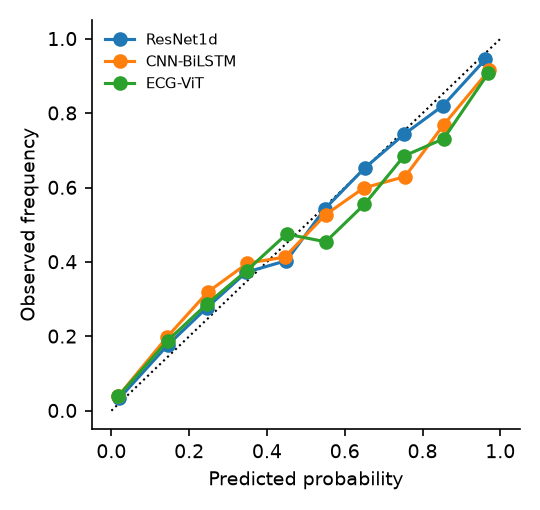
\includegraphics[width=0.45\linewidth]{fig6_reliability.png}
\caption{Reliability diagram of the 12-lead models (seed 0, all classes pooled).}
\end{figure}

\begin{figure}[H]
\centering
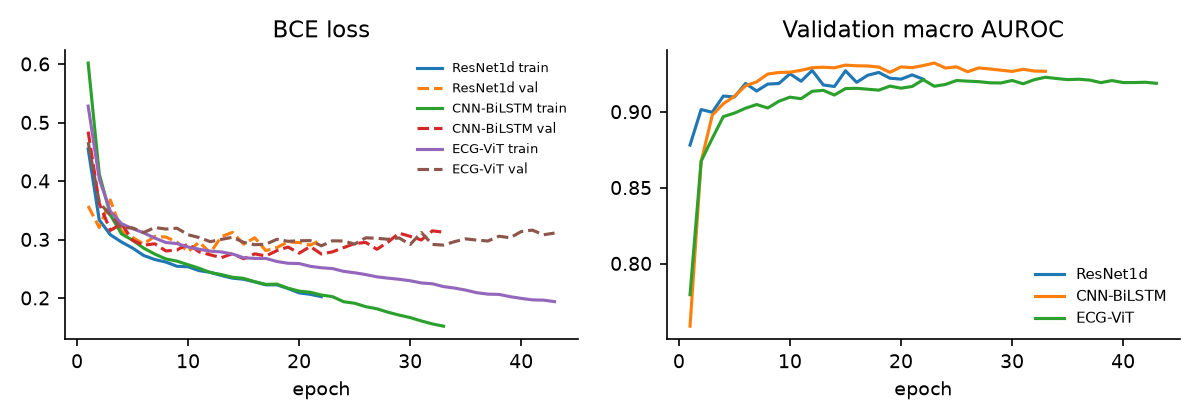
\includegraphics[width=0.85\linewidth]{fig7_training_curves.png}
\caption{Training and validation loss and validation macro AUROC of the 12-lead models (seed 0).}
\end{figure}

\begin{figure}[H]
\centering
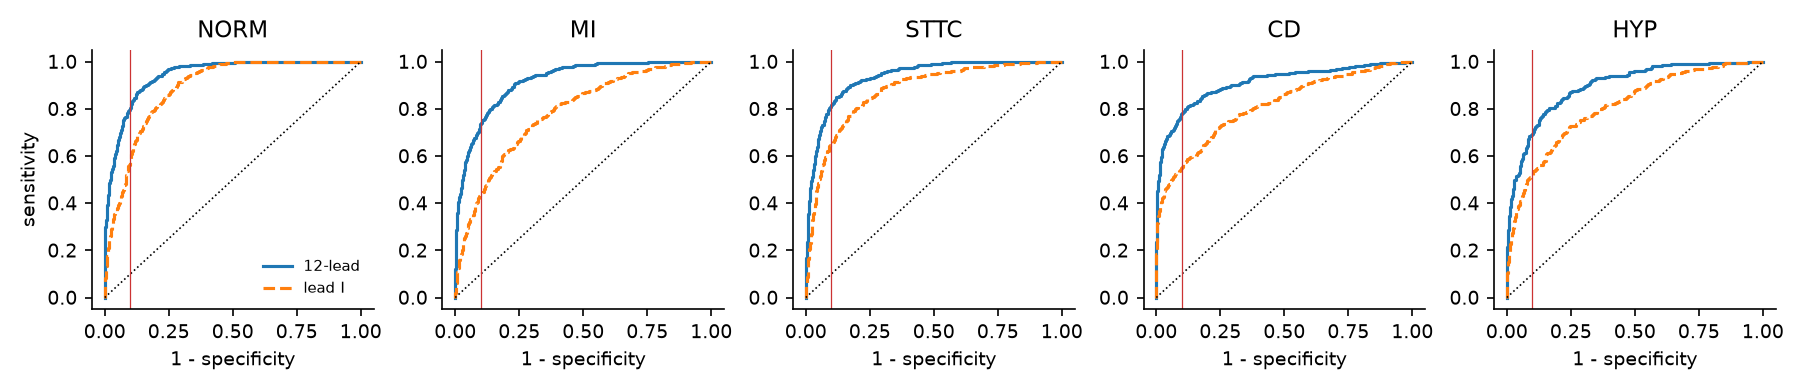
\includegraphics[width=\linewidth]{fig8_roc_12lead_vs_leadI.png}
\caption{Per-class ROC curves of ResNet1d with 12 leads and lead I (seed 0); the vertical line marks 90\% specificity.}
\end{figure}

\section{Reproducing the results}
\label{app:repro}
All code, launch scripts and result tables are in the submitted code archive. With the PTB-XL v1.0.3 data in \texttt{data/ptb-xl}, the full pipeline is:
\begin{enumerate}
  \item \texttt{python scripts/prepare\_data.py} -- build the 100\,Hz cache;
  \item \texttt{python scripts/baselines.py} -- E0 baselines B0--B2;
  \item \texttt{python scripts/run\_experiments.py --exp all} -- E1--E5 (102 runs; finished runs are skipped);
  \item \texttt{python scripts/e8\_self\_supervised.py} -- E8 pre-training and fine-tuning;
  \item \texttt{python scripts/external\_validation.py} \texttt{--data\_dir <WFDBRecords> --name chapman} -- E7;
  \item \texttt{python scripts/summarize.py}, \texttt{conclusion\_table.py}, \texttt{ensemble\_subgroup.py}, \texttt{explain.py} and \texttt{make\_paper\_figures.py} -- tables and figures.
\end{enumerate}
Exact commands, environment details and expected run times are given in the archive's \texttt{README.md}.
